\documentclass[a4paper,12pt,oneside]{article}

% Imported packages
\usepackage[english]{babel}
\usepackage[T1]{fontenc}
\usepackage[utf8]{inputenc}
\usepackage{float}
\usepackage{graphicx}
\usepackage{amssymb}
\usepackage{amsmath}
\usepackage{bm}
\usepackage{listings}
\usepackage{comment}
\usepackage{geometry}
\usepackage{wrapfig}
\usepackage{subfigure}

% Margin dimensions settings
\geometry{a4paper,top=2cm,bottom=2cm,left=2cm,right=2cm,%
	heightrounded,bindingoffset=5mm}

% Enumeration settings
\renewcommand\thesubsection{\thesection.\alph{subsection}}

% Code visualization settings
\lstset{basicstyle=\small\ttfamily}

% Code design settings
\lstset{language=Matlab}

% Included images path
\graphicspath{{Images/}}

% Document information
\title{Fundamentals of Vibration Analysis and Vibroacoustics \\
	Module 2 - Vibroacoustics of Musical Instruments \\
	Assignment 1 - Axial vibration of undamped and damped bars}
\author{Bombaci Nicola 10677942 \\
	Fantin Jacopo 10591775 \\
	Intagliata Emanuele 10544878}
\date{June 2020}


\begin{document}

\maketitle

\vspace{100pt}

\section*{System schematic and parameters}

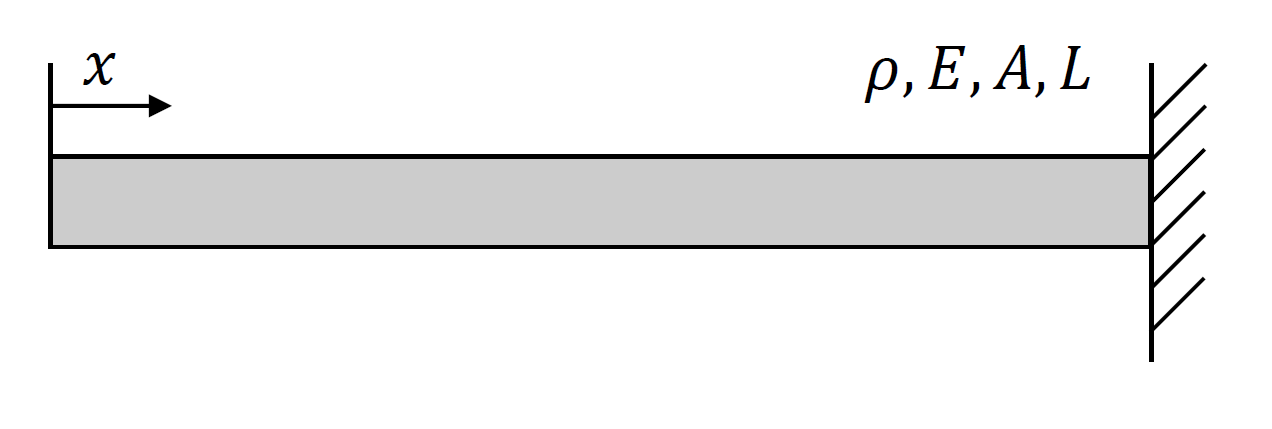
\includegraphics[width=0.9\textwidth]{system_schematic}

\vspace{30pt}

\[
	\rho = 2700 \, \text{kg/m\textsuperscript{3}} ~ \text{,} ~ E = 70 \, \text{GPa} %
		~ \text{,} ~ L = 2 \, \text{m} ~ \text{,} ~ b = h = 0.05 \, \text{m}
\]

\clearpage


\section{Natural frequencies and mode shapes in free-fixed configuration}

Starting from the one-dimensional wave equation and applying it for the axial displacement $ s(x,t) $ of point at position $ x $ at time $ t $:

\[
	\frac{\partial^2 s(x,t)}{\partial x^2} = %
		\frac{1}{c^2} \, \frac{\partial^2 s(x,t)}{\partial t^2}
\]

We already know that a solution to the equation is the standing wave expression, where space and time dependencies are separated by the mode shape function $ \Phi(x) $ and the complex exponential $ G(t) $:

\[
	s(x,t) = \Phi(x) \, G(t) = %
		\bigl(A \, sin(kx) + B \, cos(kx)\bigl) \, e^{j \omega \, t}
\]

\vspace{10pt}

The bar is in free-fixed condition, so the boundary conditions are

\[ \begin{cases}
	N(0,t) = E \, S \, \frac{\partial s(x,t)}{\partial x} \Big|_{x=0} = 0 %
		~ \Rightarrow ~ E \, S \, A \, k \, e^{j \omega \, t} = 0 %
		~ \Rightarrow ~ A = 0 ~ \text{($ k = 0 $ is a trivial solution)} \\
	s(L,t) = 0 ~ \Rightarrow ~ B \, cos(kL) = 0 ~ \Rightarrow ~ %
		k^{\textup{fr-fx}^{(i)}} = \frac{2i - 1}{2L} \pi %
		~ \text{,} ~ i = 1,2,...,\infty
\end{cases} \]

where $ S $ denotes the area of the bar's cross-section and $ N $ the normal axial load. From the second condition, the natural frequencies can be directly retrieved:

\[
	f_\textup{n}^{\textup{fr-fx}^{(i)}} = %
		\frac{\omega_\textup{n}^{\textup{fr-fx}^{(i)}}}{2 \pi} = %
		\frac{c \, k^{\textup{fr-fx}^{(i)}}}{2 \pi} = %
		\frac{2i - 1}{4L} \sqrt{\frac{E}{\rho}} ~ \text{,} ~ i = 1,2,...,\infty
\]

Our analysis is restricted to the frequency band $ [0, f_\textup{max}] = [0, 10k] \, $ Hz, so $ i $ assumes values within a finite set of indices:

\[ \begin{split}
	& f_\textup{max} = \frac{2 \, i^\textup{fr-fx}_\textup{max} - 1}{4L} %
		\sqrt{\frac{E}{\rho}} \\
	& \Rightarrow ~ \lfloor i^\textup{fr-fx}_\textup{max} \rfloor = %
		\Biggl\lfloor 2 L f_\textup{max} %
		\sqrt{\frac{\rho}{E}} + \frac{1}{2} \Biggr\rfloor = \lfloor 8.35 \rfloor = 8
\end{split} \]

So $ i = 1,2,...,8 $ and the resulting natural frequencies are

\[
	\mathbf{f_n^{fr-fx}} =	\begin{bmatrix}
														636.47		& 1909.40	& 3182.30	& 4455.30 %
														& 5728.20	& 7001.20	& 8274.10	& 9547.00
													\end{bmatrix}
\]

The mode shapes $ \Phi^{\textup{fr-fx}^{(i)}} $ are then, considering the constant coefficient $ B = 1 $,

\[
	\Phi^{\textup{fr-fx}^{(i)}} = cos(k^{\textup{fr-fx}^{(i)}} x) = %
		cos\biggl(\frac{2i - 1}{2L} \pi \, x\biggr) ~ \text{,} ~ i = 1,2,..,8
\]

We hereby show them plotting the oscillation amplitude of each point of the bar versus the points position.

\begin{figure}[h]
	\centering
	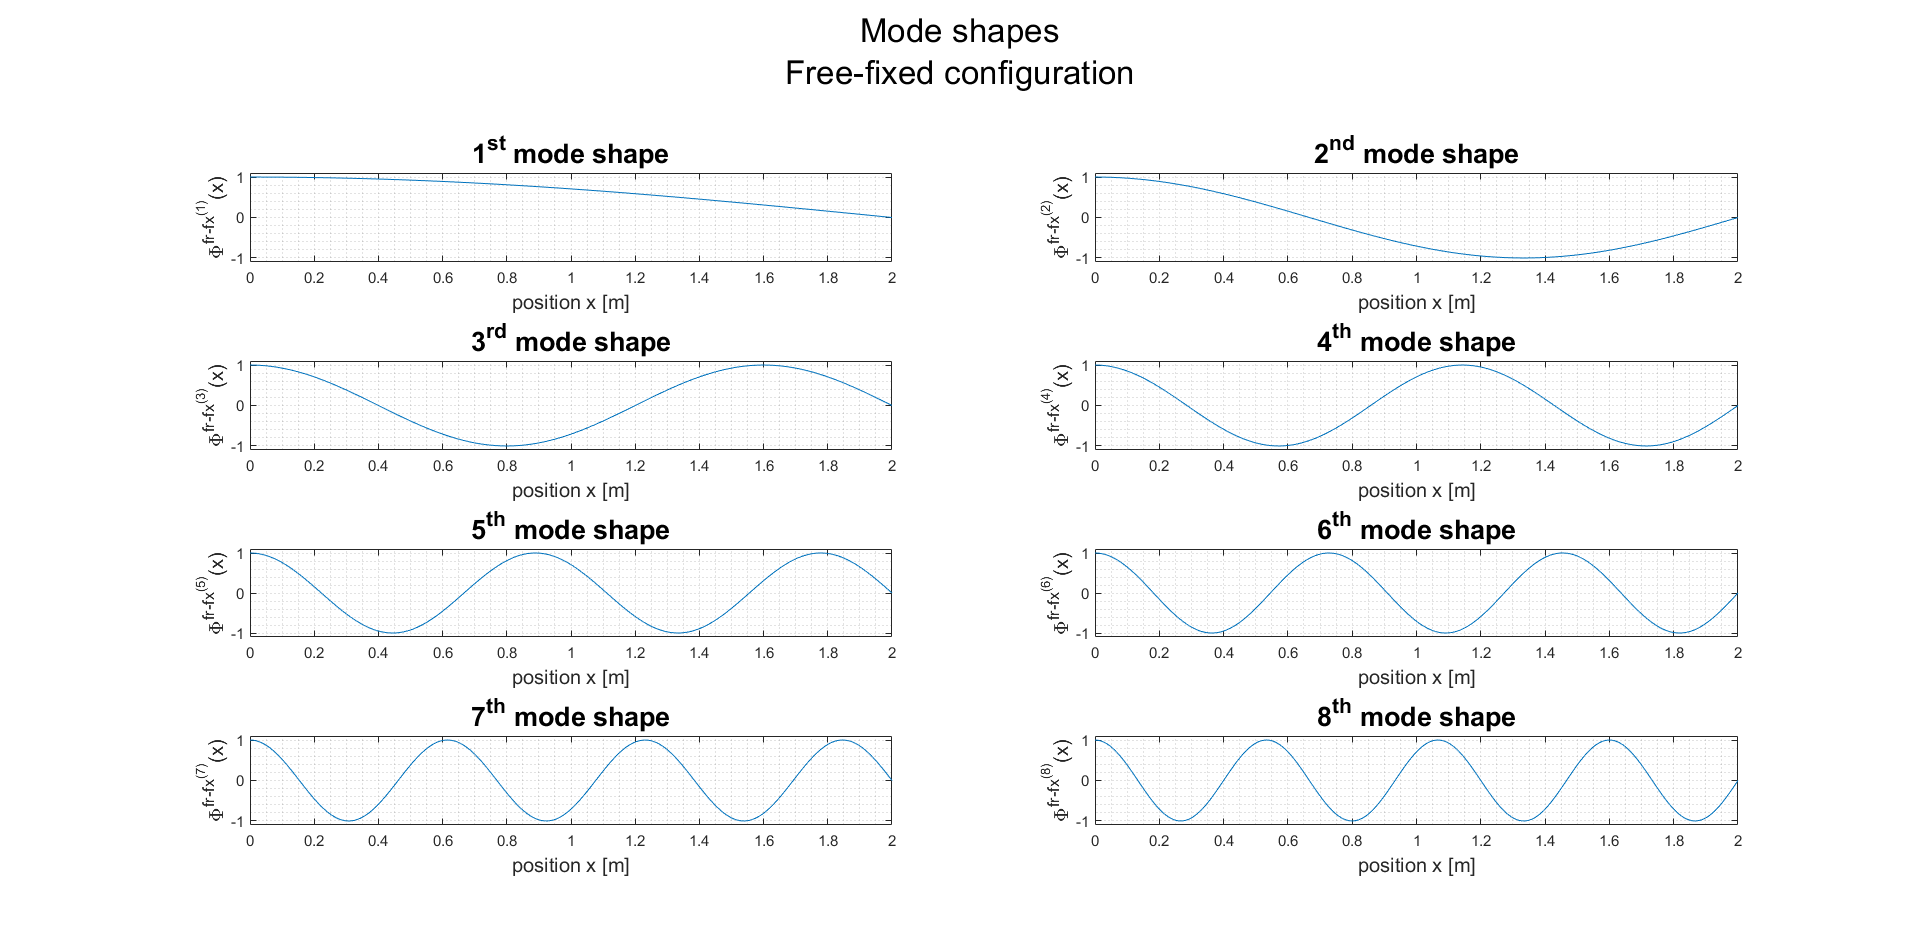
\includegraphics[scale=0.4]{mode_shapes_free_fixed}
\end{figure}


\section{Natural frequencies and mode shapes in free-free configuration}

Differently, in a free-free configuration of the bar the boundary condition on the normal force $ N $ is applied to the right end of the bar too:

\[ \begin{split}
	& \begin{cases}
			N(0,t) = E \, S \, \frac{\partial s(x,t)}{\partial x} \Big|_{x=0} = 0 %
				~ \Rightarrow ~ E \, S \, A \, k \, e^{j \omega \, t} = 0 %
				~ \Rightarrow ~ A = 0 ~ \text{($ k = 0 $ is a trivial solution)} \\
			N(L,t) = E \, S \, \frac{\partial s(x,t)}{\partial x} \Big|_{x=L} = 0 %
				~ \Rightarrow ~ - E \, S \, B \, k \, sin(kL) = 0 ~ \Rightarrow ~ sin(kL) = 0
	\end{cases}	\\
	& \hspace{150pt}~ \Rightarrow ~ %
		k^{\textup{fr-fx}^{(i)}} = \frac{i}{L} \pi ~ \text{,} ~ i = 0,1,...,\infty
\end{split} \]

So the natural frequencies are computed from $ k^{\textup{fr-fr}^{(i)}} $ as before:

\[
	f_\textup{n}^{\textup{fr-fr}^{(i)}} = %
		\frac{\omega_\textup{n}^{\textup{fr-fr}^{(i)}}}{2 \pi} = %
		\frac{c \, k^{\textup{fr-fr}^{(i)}}}{2 \pi} = %
		\frac{i}{2L} \sqrt{\frac{E}{\rho}} ~ \text{,} ~ i = 0,1,...,\infty
\]

This time the maximum value for index $ i $ is

\[ \begin{split}
	& f_\textup{max} = \frac{i^\textup{fr-fr}_\textup{max}}{2L} %
		\sqrt{\frac{E}{\rho}} \\
	& \Rightarrow ~ \lfloor i^\textup{fr-fr}_\textup{max} \rfloor = %
		\Biggl\lfloor 2 L f_\textup{max} \sqrt{\frac{\rho}{E}} \Biggr\rfloor = %
		\lfloor 7.86 \rfloor = 7
\end{split} \]

So $ i = 0,1,...,7 $ and the corresponding natural frequencies are

\[
	\mathbf{f_n^{fr-fr}} =	\begin{bmatrix}
																	0					& 1272.9	& 2545.9	& 3818.8 %
																	& 5091.8	& 6364.7	& 7637.6	& 8910.6
													\end{bmatrix}
\]

The number of resonances within $ f_\textup{max} $ is the same, but the most important consideration is about the fact the system has now a resonance at $ f = 0 $, that is, a non-oscillating mode. The second consideration is that, while in the free-fixed case the resonance frequencies are odd integer multiples of the fundamental, in the free-free case these are all the integer multiples of the fundamental, both even and odd, which is twice that of the first case. In other words, naming $ f_0 $ the fundamental frequency of the free-fixed configuration, in the first case the resonances are

\[
	\mathbf{f_n^{fr-fx}} =	\begin{bmatrix}
														f_0	& 3f_0	& 5f_0	& 7f_0	& 9f_0	& 11f_0	& 13f_0	& 15f_0
													\end{bmatrix}
\]

while in the second case

\[
	\mathbf{f_n^{fr-fr}} =	\begin{bmatrix}
														0	& 2f_0	& 4f_0	& 6f_0	& 8f_0	& 10f_0	& 12f_0	& 14f_0
													\end{bmatrix}
\]

Just like before, the resulting mode shapes $ \Phi^{\textup{fr-fr}^{(i)}} $ are computed and plotted considering $ B = 1 $.

\[
	\Phi^{\textup{fr-fr}^{(i)}} = cos(k^{\textup{fr-fr}^{(i)}} x) = %
		cos\biggl(\frac{i}{L} \pi \, x\biggr) ~ \text{,} ~ i = 0,1,...,7
\]

\begin{figure}[h]
	\centering
	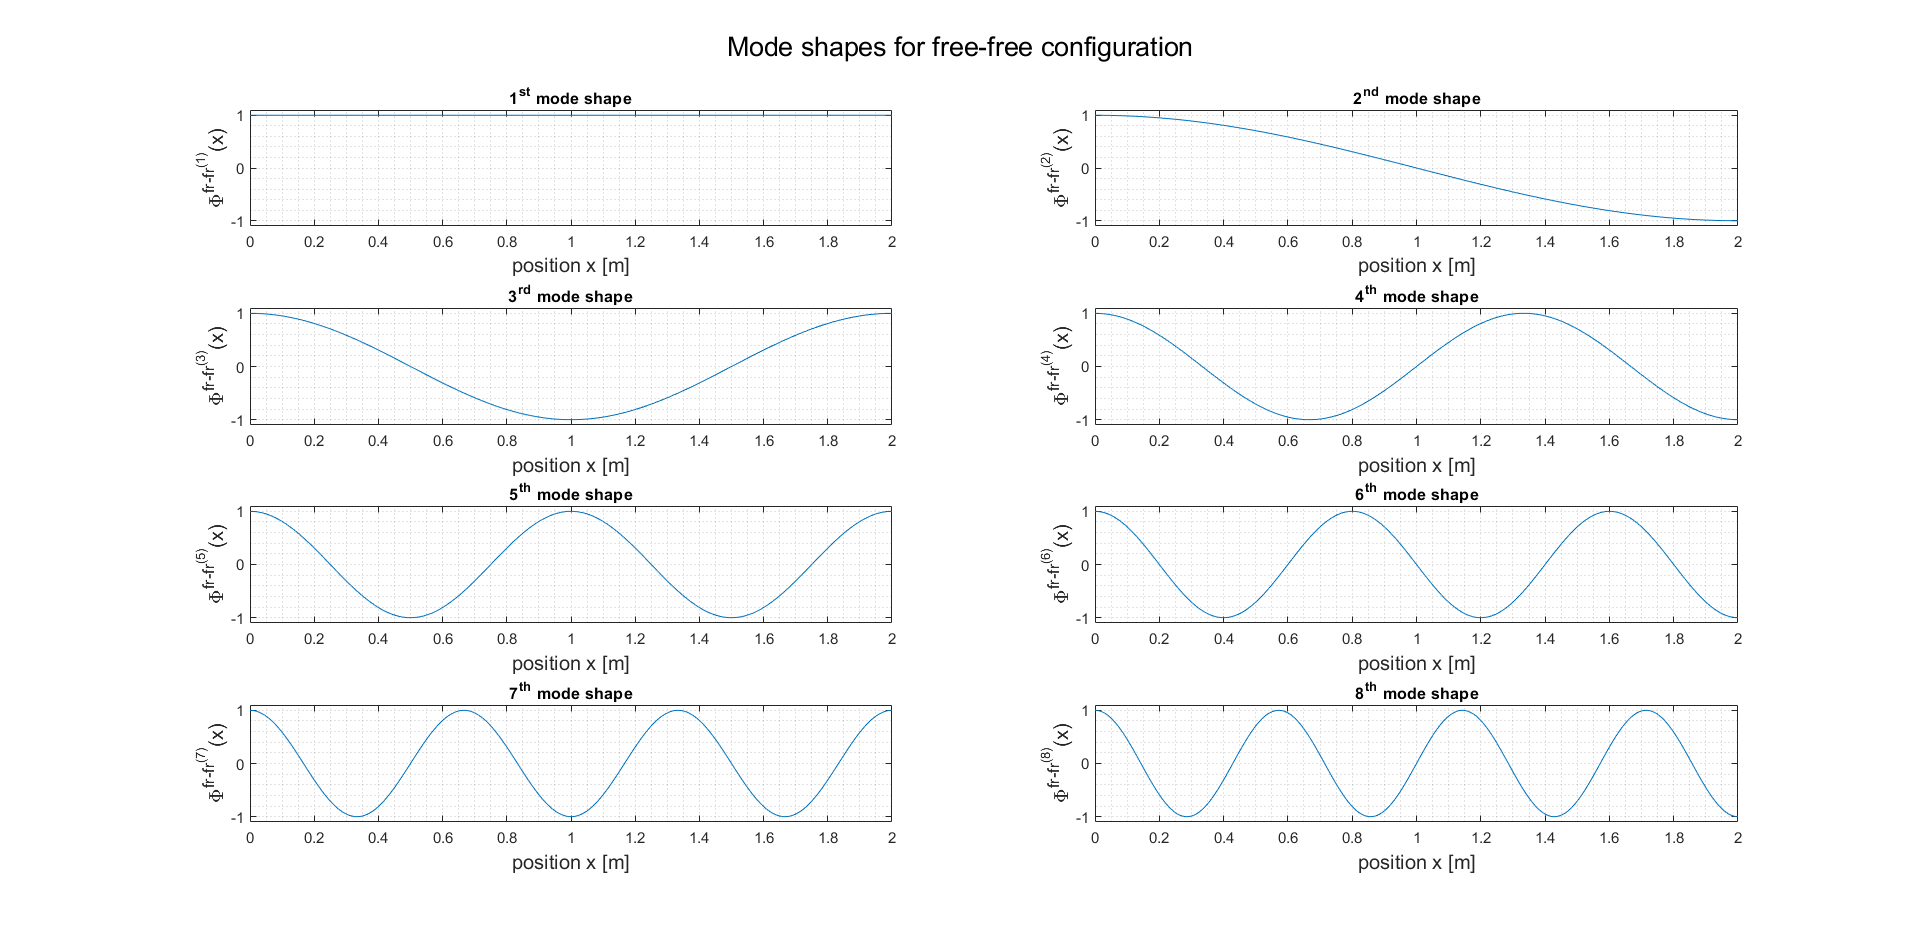
\includegraphics[scale=0.4]{mode_shapes_free_free}
\end{figure}


\end{document}
